Во {\textbf{введении}} обосновывается актуальность
исследований, проводимых в~рамках данной диссертационной работы,
приводится обзор научной литературы по~изучаемой проблеме,
формулируется цель, ставятся задачи работы, излагается научная новизна
и практическая значимость представляемой работы, приводится структура и содержание.

{\textbf{Первая глава}} посвящена обзору имеющейся литературы и постановке задачи в виде задачи математического программирования. Здесь рассматриваются источники, позволяющие сформулировать постановку задачи\mycite{sazonov:PAA,yurkov:farkv}{Сазонов~Д.М.,~1988, Юрков~А.С.,~2014}, приводится анализ аналогичных исследований~\mycite{luo:sdp,fuchs:application}{Luo~Z.,~2009, Fuchs~B.,~2014}. Также в рамках этого раздела производится сравнение результатов работы различных методов решения поставленной задачи.

В рассматриваемой в данной работе задаче требуется максимизировать излучение антенной решетки в заданном направлении при ограничениях на мощность, подводимую к каждому излучателю. В терминах комплексных токов, подводимых к излучателям, эта задача сформулирована в работах~\mycite{yurkov:farkv, yurkov:knd}{Юрков~А.С.,~2016,~2014}. Целевая функция задачи оптимизации определяется следующим образом:
%
    \begin{equation}
        F = \textbf{u}^{+}\textbf{Au} \, ,
        \label{eq:F_0}
    \end{equation}
%
где верхний индекс $+$ означает эрмитово сопряжение, $\textbf{u}$ -- вектор-столбец комплексных напряжений, подаваемых на излучатели системы, $A = (a_{ij})$,
%
     \begin{equation}
        a_{ij} = \sum_{l=1}^2\overline{f}_{i}^{(l)}f_{j}^{(l)}
        \label{eq:A_0} \, .
    \end{equation}
%
%https://mash-xxl.info/page/237228250236048025008225022139044243122210140103/
Здесь $f_i^{(l)}$ -- парциальное поле, то есть поле, которое излучается при подаче единичного тока на $i$-ю точку питания излучающей системы, в то время, как ток в других точках питания равен нулю.

В данной работе рассматривается случай, когда ограничение на мощность накладывается по каждой точки питания. В случае ограничения суммарной мощности, подаваемой на антенную систему, задача может быть решена аналитически~\mycite{yurkov:farkv}{Юрков~А.С., 2014}. В других постановках ограничения накладываются не на мощность, а на излучение~\mycite{fuchs:application}{Fuchs~B.,~2014}. В рассматриваемом здесь случае задача формулируется в виде:
%
    \begin{equation}
        \begin{cases}
           \textbf{u}^{+}\textbf{Au} \rightarrow \max,\\
           0 \leq \textbf{u}^{+}\textbf{B}^{(1)}\textbf{u} \leq 1, \\
           ...\\
           0 \leq \textbf{u}^{+}\textbf{B}^{(n)}\textbf{u} \leq 1,\\
           \textbf{u} \in \mathbb{C}^N\\
         \end{cases}
         \label{eq:task2_0}
    \end{equation}
%
где $\mathbb{C}$ -- поле комплексных чисел, $n$ -- число точек питания, на которые накладываются ограничения (в общем случае $n$ может быть не равно $N$),
%
    \begin{equation}
        \textbf{B}^{(k)} = \frac{1}{4P_{max}^{(k)}}(\textbf{Y}^{+}\mathcal{P}^{(k)} + \mathcal{P}^{(k)}\textbf{Y}) \, ,
    \end{equation}
%
$P_{max}^{(k)}$ -- максимально допустимая мощность в $k$-й точке питания, $\mathcal{P}^{(k)}$ -- матрицы-проекторы имеющие единственный ненулевой элемент $\mathcal{P}^{(k)}_{kk}=1$. Матрицы-проекторы имеют размерность $N \times N$. Поскольку аргументом целевой функции является вектор комплексных токов, задачу оптимизации направленности ФАР КВ диапазона также можно назвать задачей оптимизации фаз и амплитуд. За $\textbf{Y}$ обозначается матрица проводимостей.

Следует отметить, что задача~(\ref{eq:task2_0}), сформулированная в комплексных числах, имеет симметрию относительно преобразования $\textbf{u} \to e^{\emph{\textbf{j}}\phi}\textbf{u}$ всех комплексных координат (по произвольному углу~$\phi$). За $\emph{\textbf{j}}$ здесь обозначена мнимая единица. Данная симметрия может найти применение для уменьшения размерности области поиска на единицу. Например, фиксируя $Im(y_{N})=0$, что эквивалентно добавлению ограничения $x_{2N}=0$ к задаче~(\ref{eq:task3_0}).

Для разработки алгоритма решения задачи удобно переформулировать ее в вещественных числах. В вещественных числах задача~(\ref{eq:task2_0}) эквивалентна следующей:
        \begin{equation}
            \begin{cases}
               \textbf{x}^{T}\textbf{Gx} \rightarrow \max,\\
               0 \leq \textbf{x}^{T}\textbf{H}^{(1)}\textbf{x} \leq 1,\\
               ...\\
               0 \leq \textbf{x}^{T}\textbf{H}^{(n)}\textbf{x} \leq 1,\\
              \textbf{x} \in \mathbb{R}^{2N}.\\
             \end{cases}
             \label{eq:task3_0}
        \end{equation}

Задача~(\ref{eq:task3_0}) имеет целевую функцию, заданную квадратичной формой с положительно полуопределенной матрицей~$\textbf{G}$. Каждое ограничение формулируется квадратичной формой, определенной симметричной матрицей~$\textbf{H}^{(k)}, k=\overline{1,n}$ с двумя парами идентичных собственных значений, два из которых положительны, а другие два отрицательны или равны нулю, все остальные собственные числа равны нулю.

Для задачи~(\ref{eq:task3_0}) существует преобразование, позволяющее привести к допустимой области решение $\textbf{x}$, которое нарушает только ограничивающие неравенства задачи~(\ref{eq:task3_0}) вида $\textbf{x}^{T}\textbf{H}^{(k)}\textbf{x} \leq 1$:

\begin{equation}
    \textbf{x}': =\alpha(\textbf{x})^{-1/2} \textbf{x} ,
    \label{eq:scale_0}
\end{equation}
где $\alpha(\textbf{x}):=\max_{k=\overline{1,n}} \textbf{x}^T \textbf{H}^{(k)}\textbf{x}$. Данная процедура применяется для выбора начального решения, а также для масштабирования итогового решения градиентного подъема и может использоваться  в дифференциальной эволюции.

В вычислительных экспериментах бывает полезно ограничить множество допустимых решений задачи шаром или параллелепипедом, так как это позволяет более обоснованно выбрать начальное решение для итерационных методов с мультистартом или сократить перебор в методе ветвей и границ. Отметим, что если вектор $\textbf{x}$ удовлетворяет всем ограничениям задачи~(\ref{eq:task3_0}), то
\begin{equation} \label{eqn:bound}
||\textbf{x}||\le \sqrt{\frac{N}{\lambda_{\min}}}.
\end{equation}

Глобально-оптимальное решение задачи невыпуклого математического программирования вида (\ref{eq:task3_0}) может быть найдено методом
ветвей и границ~\mycite{horst:global,tawarmalani:global}{Horst~R.,~2013, Tawarmalani~M.,~2004} или с использованием методов DC программирования~\mycite{horst:handbook,strekalovsky:global}{Horst~R.,~2013, Strekalovsky~А.С.,~2007}. Локально-оптимальное решение задачи может быть найдено средствами градиентной оптимизации или методом Ньютона. В случае большой размерности могут быть применены различные метаэвристики~(см.~\mycite{eberhart:swarm,storn:de}{Eberhart~R,~1995., Storn~R.,~1997}).

Процедура решения задачи оптимизации ФАР при ограничении мощности по каждой точке питания состоит в следующем:
%
\begin{enumerate}
  \item Для каждого излучателя в решетке рассчитать парциальные компоненты полей $f_i^{(l)}, i= \overline{1,N}, l=\overline{1,2}$.
  \item Вычислить матрицы $\textbf{G}$ and ${\textbf{H}}^{(k)},\ k=\overline{1,n}$.
  \item Оценить радиус допустимой области.
  \item Решить задачу~(\ref{eq:task3_0}) с дополнительными ограничениями $x_N = 0, ||\textbf{x}||\le \sqrt{\frac{N}{\lambda_{\min}}}$.
\end{enumerate}

Данный подход может гарантировать нахождение как локального, так и глобального оптимума, в зависимости от решателя, используемого на шаге~4. Как один из базовых оптимизационных методов, в главе 1 мы рассматриваем метод градиентной оптимизации (максимизационный вариант)
с алгоритмом одномерного поиска Дэвиса, Свенна и Кэмпи~(ДСК)~\mycite{himmelblau:nlp}{Himmelblau~D.M.,~1972}. Далее целевая функция задачи~(\ref{eq:task3_0}) будет обозначатся символом $\tilde{F}$.

В нашей работе от задачи условной оптимизации мы переходим к задаче безусловной оптимизации методом штрафных функций, а именно -
методом внешней точки~\mycite{eremin:convex,aoki:mo}{Еремин~B.B.,~1976, Aoki~M.,~1971}:
\begin{equation}
       \textbf{x}^{T}\textbf{Gx} - r\cdot \sum_{k=1}^n
       \left( \min\left(0,\textbf{x}^{T}\textbf{H}^{(k)}\textbf{x}\right) +
       \min\left(0,1-\textbf{x}^{T}\textbf{H}^{(k)}\textbf{x}\right)\right)^4 \rightarrow
       \max,
     \label{eq:task4}
\end{equation}
где $r$ - достаточно большой штрафной параметр. Алгоритм градиентной оптимизации повторяется многократно, при этом используется случайно сгенерированный вектор~$\textbf{x}\in \mathbb{R}^{2N}$ в качестве стартовой точки.

Для организации вычислительных экспериментов был разработан программный комплекс <<Expi>>\ifdisser{(~см.~\hyperref[sec:applic_b]{приложение Б})}{}, зарегистрированный в государственном реестре программ для ЭВМ~\cite{expi}.
Вычислительный эксперимент был поставлен для задач, построенных на основе следующих типов ФАР, выпускаемых серийно и представляющих интерес для промышленности: широкополосных вертикальных излучателей~(ШВИ), широкополосных вертикальных диполей~(ШВД) и симметричных вертикальных диполей~(СВД). При моделировании полей был использован пакет NEC2, для которого были предоставлены соответствующие геометрические конфигурации антенных систем. В качестве рабочей частоты было выбрано 5МГц. Рассмотрены квадратные ФАР конфигурации 2x2, 3x3 и 5x5. Конфигурация 5x5 была рассмотрена только для решеток СВД, поскольку NEC2 не смог обработать 5x5~ШВИ и 5x5~ШВД из-за высокой сложности этих моделей. В случае с ФАР кольцевой структуры были рассмотрены решетки, состоящие из 8 и 16 излучателей. Также в рассмотрение были приняты укороченные СВД с длиной плеча 5м. (СВД'). В качестве направления максимизации излучения выбраны: азимутальный угол $45^{\circ}$, полярный угол $70^{\circ}$.

\begin{figure}
    \begin{minipage}[h]{0.49\linewidth}
        \center{\includegraphics[width=1\linewidth]{2x2bvm.eps} \\ а)}
    \end{minipage}
    \hfill
    \begin{minipage}[h]{0.49\linewidth}
        \center{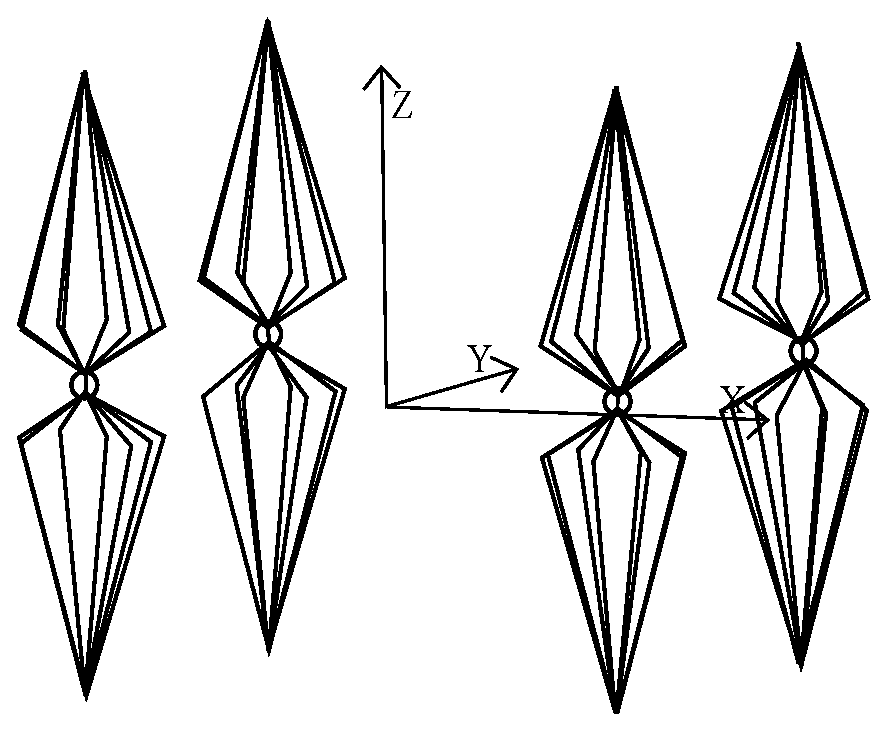
\includegraphics[width=0.6\linewidth]{2x2bvd.eps} \\ б)}
    \end{minipage}
    \begin{minipage}[h]{0.49\linewidth}
        \center{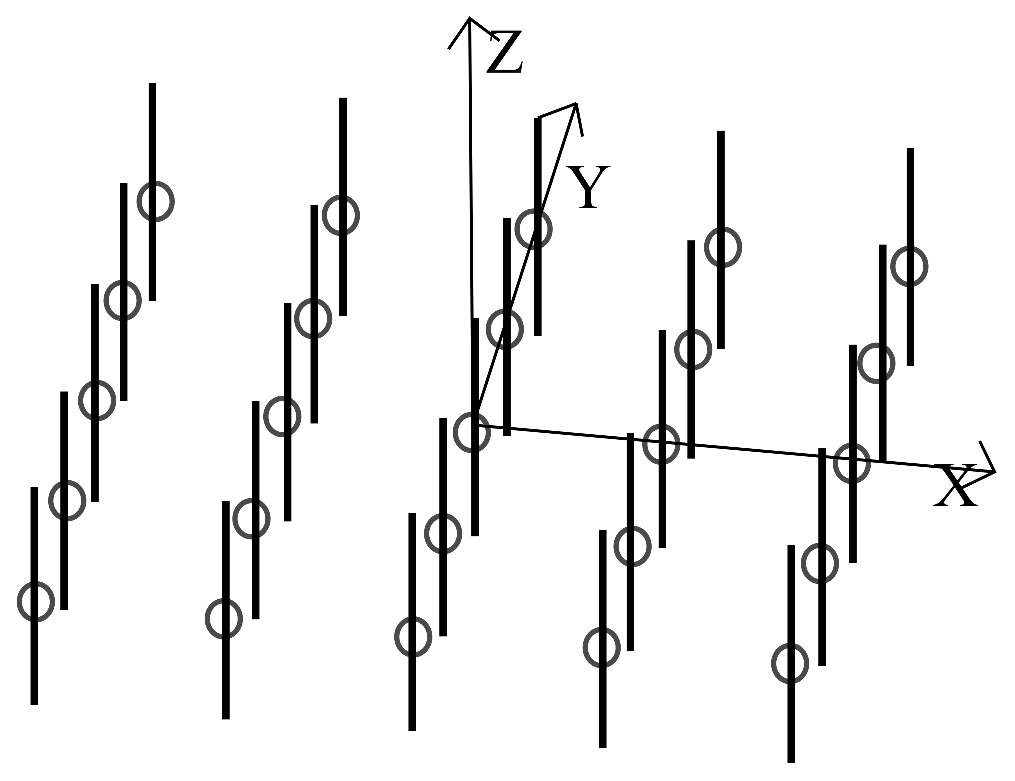
\includegraphics[width=0.6\linewidth]{5x5SVD.eps} \\ в)}
    \end{minipage}
    \hfill
    \begin{minipage}[h]{0.49\linewidth}
        \center{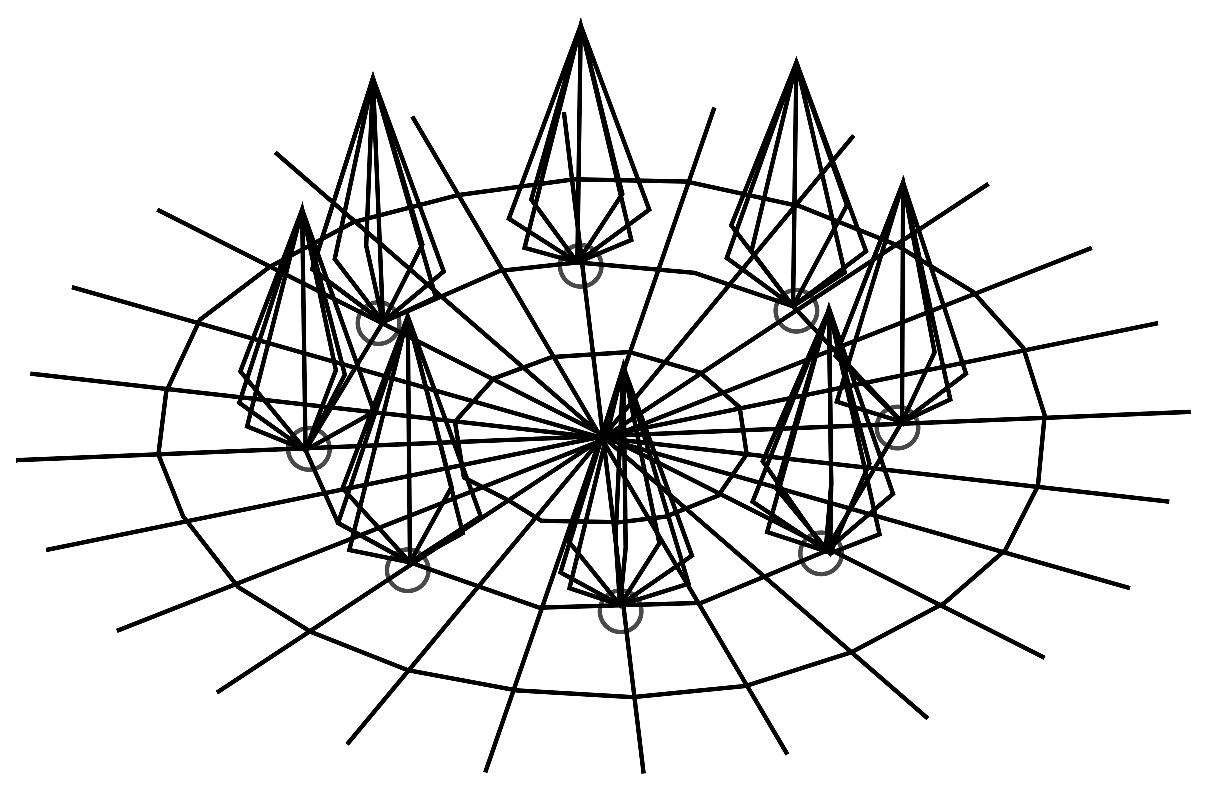
\includegraphics[width=0.9\linewidth]{r8.eps} \\ г)}
    \end{minipage}
    \caption{ФАР различных конфигураций}
    \label{ris:paas_0}
\end{figure}

Здесь сравниваются результаты работы градиентного метода и решателя BARON в его режиме по умолчанию. Во всех экспериментах, описанных ниже, было установлено ограничение по времени 1000с. Сравнение алгоритмов, представляющих принципиально различные методы, по количеству вычислений целевой функции не является корректным, поэтому, в данной работе идет сравнение именно по времени. Все эксперименты проводились на ЭВМ с процессором Intel i7 (тактовая частота: 2.8ГГц), ОЗУ: 16Гб. В случае остановки градиентного метода (завершение по минимально допустимому приращению целевой функции $10^{-4}$), алгоритм перезапускается заново до истечения запаса времени.

Во время каждой инициализации градиентного метода в главе 1 стартовая точка~$\textbf{x}$ выбирается независимо с равномерным распределением в кубе $[-5000, 5000]^{2N}$. Лучшее из найденных таким образом решений принимается за конечный результат. Параметр штрафа~$r$ в методе градиентной оптимизации установлен равным $10^6$ на всех запусках. Такое значение было определено эмпирически. В таблице~\ref{tab:results_0} приводятся результаты вычислительного эксперимента. Значения целевой функции ``$\tilde{F}$''в точке, полученной алгоритмом градиентного подъема, приводятся после процедуры масштабирования~(\ref{eq:scale_0}). Для решателя BARON версии~18.5.8 было выбрано то же самое ограничение сверху на процессорное время, что и для градиентного метода (группа колонок ``BARON''). Во всех таблицах, колонка ``t'' содержит время до получения лучшего найденного решения или до установления глобальной оптимальности. Во всех запусках градиентного метода были получены решения, где активными оказались все ограничения вида $\textbf{x}^{T}\textbf{H}^{(k)}\textbf{x} \leq 1$ и только они.

%Как было показано выше, градиентный метод может предоставить решение, не являющийся локальным оптимумом, если целевая функция слабо изменяется в окрестности текущей точки. Алгоритм дифференциальной эволюции не подвержен такому поведению. Эксперименты показывают, что в целом эволюция популяции соответствует динамике случайного облака точек, движущегося как целое вдоль рельефа оптимизируемой функции, повторяя его характерные особенности. В случае попадания в овраг «облако» принимает форму этого оврага и распределение точек становится таким, что математическое ожидание разности двух случайных векторов оказывается направленным вдоль длинной стороны оврага. Это обеспечивает быстрое движение вдоль узких вытянутых оврагов, тогда как для градиентных методов в аналогичных условиях характерно колебательная динамика «от стенки к стенке». Приведенные эвристические соображения иллюстрируют наиболее важную и привлекательную особенность алгоритма ДЭ — способность динамически моделировать особенности рельефа оптимизируемой функции. Именно этим объясняется замечательная способность алгоритма быстро проходить сложные овраги, обеспечивая эффективность даже в случае сложного рельефа.

\begin{table}[!h]
\centering
\caption{ Результаты оптимизации, полученные с помощью градиентного подъема, решателя BARON и ДЭ.}
\begin{tabular}{|c|c|c c|c c|c|}
    \hline
    \multirow{2}{*}{\textbf{Тип}} & \multirow{2}{*}{$\sqrt{\frac{N}{\lambda_{\min}}}$} & \multicolumn{2}{c}{\textbf{Град.}} & \multicolumn{2}{|c|}{\textbf{BARON}} & \textbf{ДЭ}\\
    & & \textbf{$\tilde{F}$} & \textbf{t, c} & \textbf{$\tilde{F}$} & \textbf{t, c} & \textbf{$\tilde{F}$} \\
    \hline
    ШВИ 2х2 & 13.6 & 138 & {0.054} & {139} & 0.12 & {139}  \\
    ШВИ 3х3 & 22.5 & 576 & 0.93 & {581} & {0.34} & {581}  \\
    ШВД 2х2 & 21 & 460 & {0.13} & {464} & 0.27 &  {464}  \\
    ШВД 3х3 & 82.2 & 915 & 24.4 & {925} & {0.34} & 924   \\
    СВД 2х2 & 44.7& 357 & 1.9 & {361} & {0.16} & {361}   \\
    СВД 3х3 & 641.9& 1138 & 25.6 & \textbf{1261} & {0.38} & 1163 \\
    СВД 5х5 & $1.1\cdot10^{5}$ & 5318 & 1000 & 6716 & 1000 & \textbf{7132}  \\
    СВД' 2х2 & $2.3\cdot10^{4}$ & 233 & 2.52 & \textbf{253} & {0.25} & 198  \\
    СВД' 3х3 & $6\cdot10^5$& 664 & 71 & \textbf{1153} & {1.48} & 834  \\
    СВД' 5х5 & - & 1382 & 1000 & 33.5 & 217.94 & \textbf{2755}   \\
    Кольц. 8 & 87 & 217 & 8.06 & 218 & {0.23} & 218  \\
    Кольц. 16          & 154 & 727 & 90.9 & 734 & {1.37} & 732  \\
    \hline
\end{tabular}
\label{tab:results_0}
\end{table}

Из таблицы~\ref{tab:results_0} видно, что на всех видах решеток, кроме решеток СВД конфигураций~3x3 и~5x5, а также СВД' конфигураций~2x2 и~3x3, разница в значениях целевой функции не превосходит 1\%. Для решеток СВД конфигураций~3x3 и~5x5, а также СВД' конфигураций~2x2 и~3x3 градиентный алгоритм существенно уступает по качеству найденного решения. Кроме решeток ШВИ и ШВД конфигурации~2x2 BARON демонстрирует лучшее время счета.

Cледует отметить, что для обоих алгоритмов время, затраченное на поиск решения, было либо существенно меньше, либо сравнимо со временем, затраченным на построение исходных данных пакетом моделирования NEC, что делает оба подхода равноценными по времени работы с практической точки зрения. При увеличении времени счета BARON до 50000c. для ФАР конфигураций ШВИ~2x2, ШВД~2x2 и ШВИ~3x3 была доказана глобальная оптимальность найденного решателем BARON решения из таблицы~\ref{tab:results_0}.
%Также показано, что использование комбинированного алгоритма, сочетающего ДЭ и градиентный подъем с адаптацией штрафа, предоставляет не худшие результаты, чем градиентный метод, а в некоторых случаях, даже лучшие, чем BARON. Однако, завершение алгоритма ДЭ требует существенно больше времени.
Решатель ANTIGONE, разработанный для решения многоэкстремальных задач математической оптимизации, также был опробован в режиме его настроек по умолчанию, но в большинстве тестовых примеров возвращал нулевое решение, которое является стационарной точкой, но не является локальным оптимумом.

Во {\textbf{второй главе}} производится исследование возможности оптимизации поставленной задачи методами дифференциальной эволюции.

Очевидным недостатком градиентного подъема является невозможность выйти из окрестности локального оптимума. Таким образом, данный алгоритм хорошо подходит лишь для работы в режиме мультистарта или же для уточнения некоторого заданного решения. Такое решение может быть получено алгоритмом дифференциальной эволюции (ДЭ), который  демонстрирует хорошие результаты на различных задачах~(см., например,~\mycite{das:de}{Das~S.,~2011}) и в комбинации с градиентным алгоритмом может рассматриваться как альтернатива мультистарта.

Кратко опишем идею алгоритма. В начале происходит генерация популяции. Если нет дополнительной информации, особи популяции генерируются случайным образом с равномерным распределением. Затем, каждая особь подвергается мутации путем присваивания ей признаков другой особи.
Для этого случайным образом выбираются неравные друг другу особи $A$, $B$, $C$. Из них формируется новая особь $C' = C + f(A - B)$, где $f$ -- параметр алгоритма. Из исходной особи и особи $C'$ формируется особь новой популяции. Для этого каждый признак исходной особи с заданной вероятностью $p$ заменяются на соответствующий признак $C'$. Выживает особь с лучшим значением целевой функции.

%В данной работе был предложен вариант реализации алгоритма дифференциальной эволюции, адаптированный для запуска на графическом устройстве.
В данной работе была предложена модификация алгоритма, при которой к особи с лучшим значением целевой функции применяется градиентный алгоритм, если количество итераций алгоритма превышает двухкратное количество итераций, потребовавшееся для получения текущего рекорда~\mycite{HK93}{Hampson~S,~1996}. По истечении заданного количества итераций к лучшему решению также применяется градиентный подъем.
%При таком подходе гарантируется сходимость алгоритма к локальному оптимуму, что может не произойти в реализации алгоритма ДЭ.
%Использование алгоритма ДЭ позволило достичь решения с целевой функцией $\tilde{F} = 253$ для задачи СВД'~2x2.

Алгоритм ДЭ сравнивался с решателем BARON на пяти задачах из гл.~4~(ШВИК~8-15(2:3), ШВДК~8-20, ШВДК~8-30, СВДК~8-25, СВДК~8-37) в тех же условиях, что описаны выше. Алгоритм ДЭ на всех примерах нашел допустимые решения, а решатель BARON -- только в четырех примерах. На этих примерах результаты ДЭ отличались не более чем на~1\% по целевой функции от решений BARON. С точки зрения практики радиосвязи КВ диапазона такое отклонение пренебрежимо мало. Из проведенных экспериментов можно сделать вывод о том, что разработанный гибридный вариант ДЭ показывает конкурентоспособные результаты в сравнении с коммерческим решателем BARON в режиме его настроек по умолчанию, при этом преимущество ДЭ наблюдается на задачах с наибольшей размерностью.

{\textbf{Третья глава}} посвящена исследованию структуры локальных оптимумов с помощью различных алгоритмов оптимизации,
производится анализ наличия групп непрерывных симметрий.

Для оценки общего числа локальных оптимумов использовался метод переписи Шнабеля. Данный метод имеет применение в экологии и заключается в
выводе статистических оценок численности популяции на основе числа особей, помеченных в результате эксперимента, из популяции с неизменным
составом. В~\mycite{reves_eremeev}{Reeves~C.R., Eremeev~A.V., 2004} предлагается адаптация такого метода для оценки числа локальных оптимумов. В таблице~\ref{tab:structure_0} приводится статистика по числу различных точек остановки (в пределах заданной точности) процедуры мультистарта в течение 1000~с. процессорного времени. Для каждого решения была применена процедура линеаризации задачи и проверки необходимых условий локальной оптимальности. Здесь {$M$} -- число выполненных запусков за отведенное время, $M_{ne}$ -- число групп решений, отличающихся не более чем на 10\% по каждой из координат, {$M_{f}$} -- число групп значений целевой функции у таких неэквивалентных решений (с точностью до 10\%, приведенных в таблице~\ref{tab:results_0}). {$M_{y\approx0}$} -- число групп решений, для которых были выполнены необходимые условия локальной оптимальности. $\mathcal{B}$ и $\mathcal{L}$ -- оценка нижней границы и оценка максимального правдоподобия числа локальных оптимумов, рассчитанные по методу переписи Шнабеля. Доверительная вероятность для данного метода была выбрана равной 0.95. Оценки для числа решений с различными значениями целевой функции обозначены $\mathcal{B}_{M_f}$ и $\mathcal{L}_{M_f}$. Оценки для числа решений, для которых были выполнены необходимые условия локальной оптимальности, обозначены $\mathcal{B}_{M_{y\approx0}}$ и $\mathcal{L}_{M_{y\approx0}}$.


\begin{table}[!h]
\centering
\caption{Структура множества локальных оптимумов.}
\begin{tabular}{|l | l l | c c c | c c c|}
    \hline
    \textbf{ФАР} & \textbf{$M$} & \textbf{$M_{ne}$} & \textbf{$M_{f}$} & \textbf{$\mathcal{B}_{M_f}$} & \textbf{$\mathcal{L}_{M_f}$} & \textbf{$M_{y\approx0}$} & \textbf{$\mathcal{B}_{M_{y\approx0}}$} & \textbf{$\mathcal{L}_{M_{y\approx0}}$}\\
    \hline
    ШВИ 2x2 & 18368 & 4 & 1 & 1 & 1 & 4 & 4 & 4\\
    ШВД 2x2 & 7678  & 4 & 1 & 1 & 1 & 4 & 4 & 4\\
    СВД 2x2  & 523  & 1 & 1 & 1 & 1 & 1 & 1 & 1\\
    СВД 3x3  & 39  & 9 & 2 & 2 & 2 & 5 & 5 & 5\\
    СВД' 2x2  & 396  & 370 & 3 & 3 & 3 & 338 & 1000 & 1213\\
    СВД' 3x3  & 14  & 14 & 3 & 3 & 3 & 1 & 1 & 1\\
    ШВИ 3x3 & 1070  & 3 & 1 & 1 & 1 & 3 & 3 & 3 \\
    ШВД 3x3 & 41  & 4 & 4 & 4 & 4 & 1 & 1 & 1 \\
    Кольц. 8 & 124  & 9 & 2 & 2 & 2 & 9 & 9 & 9\\
    Кольц. 16 & 11  & 6 & 1 & 1 & 1& 6 & 6 & 6\\
    \hline
\end{tabular}
    \label{tab:structure_0}
\end{table}

На рис.~\ref{ris:fit_dist_0} приведены диаграммы найденных локальных оптимумов, где по оси ординат отложены значения целевой функции, а по оси абсцисс -- расстояние до лучшего известного решения. В случае а) точками обозначены результаты для кольцевых решеток, состоящих из 8 излучателей, ромбами -- для кольцевых решеток, состоящих из 16 излучателей, пятиугольниками - для СВД~3x3. В случае б) точками обозначены результаты для СВД'~2x2, ромбами -- для СВД'~3x3. Диаграмма показывает, что значения, соответствующие одному и тому же значению целевой функции, могут находиться достаточно далеко друг от друга, что позволяет сделать предположение о наличии неучтенных симметрий задачи.

\begin{figure}
\centering
    \begin{minipage}[h]{0.8\linewidth}
            \center{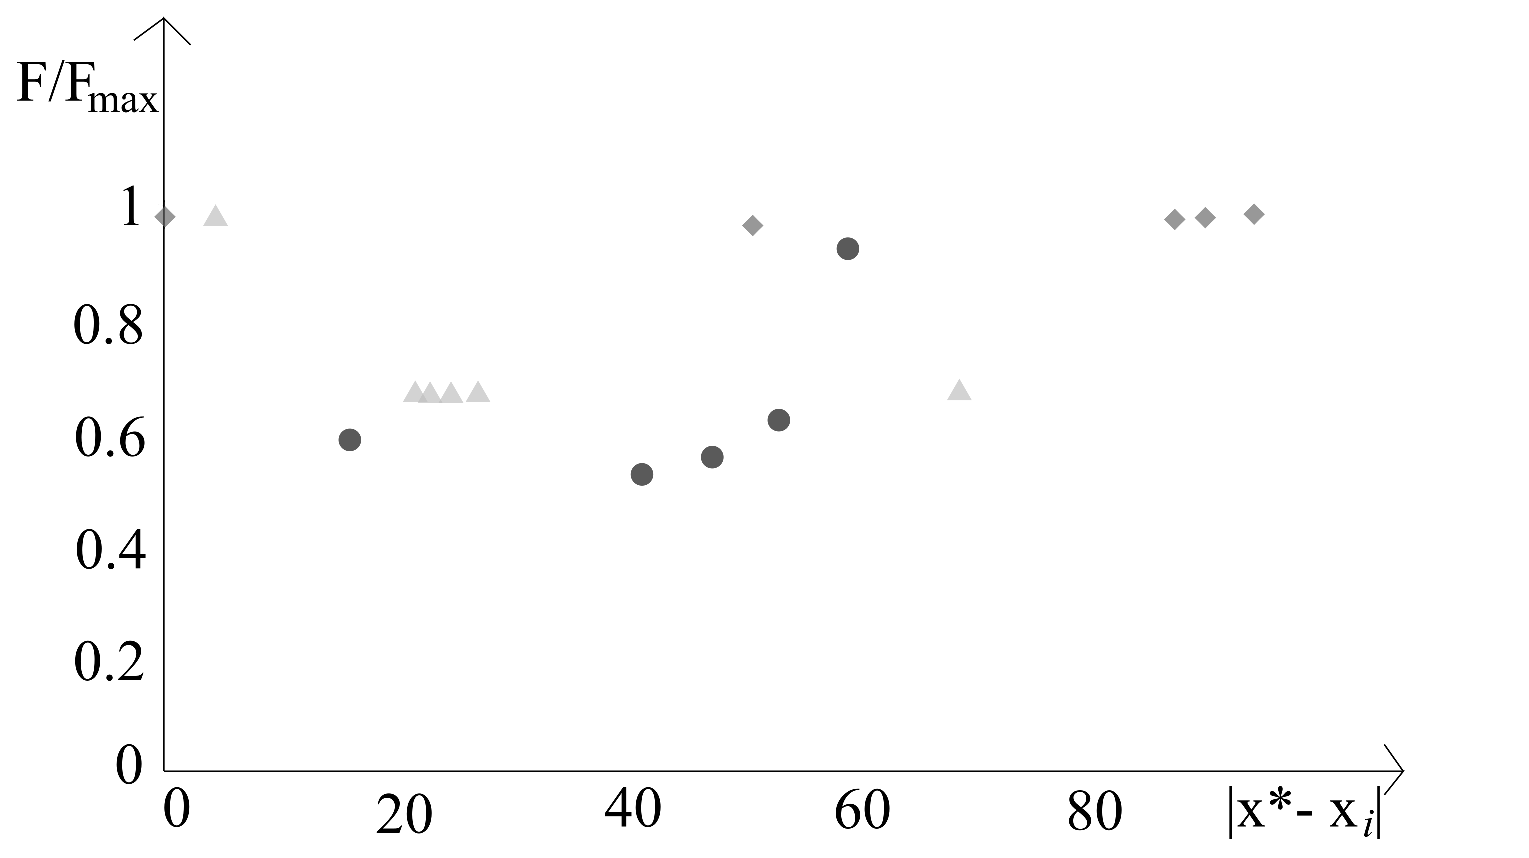
\includegraphics[width=0.9\linewidth]{fit_dist.eps}  \\ а) }
    \end{minipage}
    \begin{minipage}[h]{\linewidth}
            \center{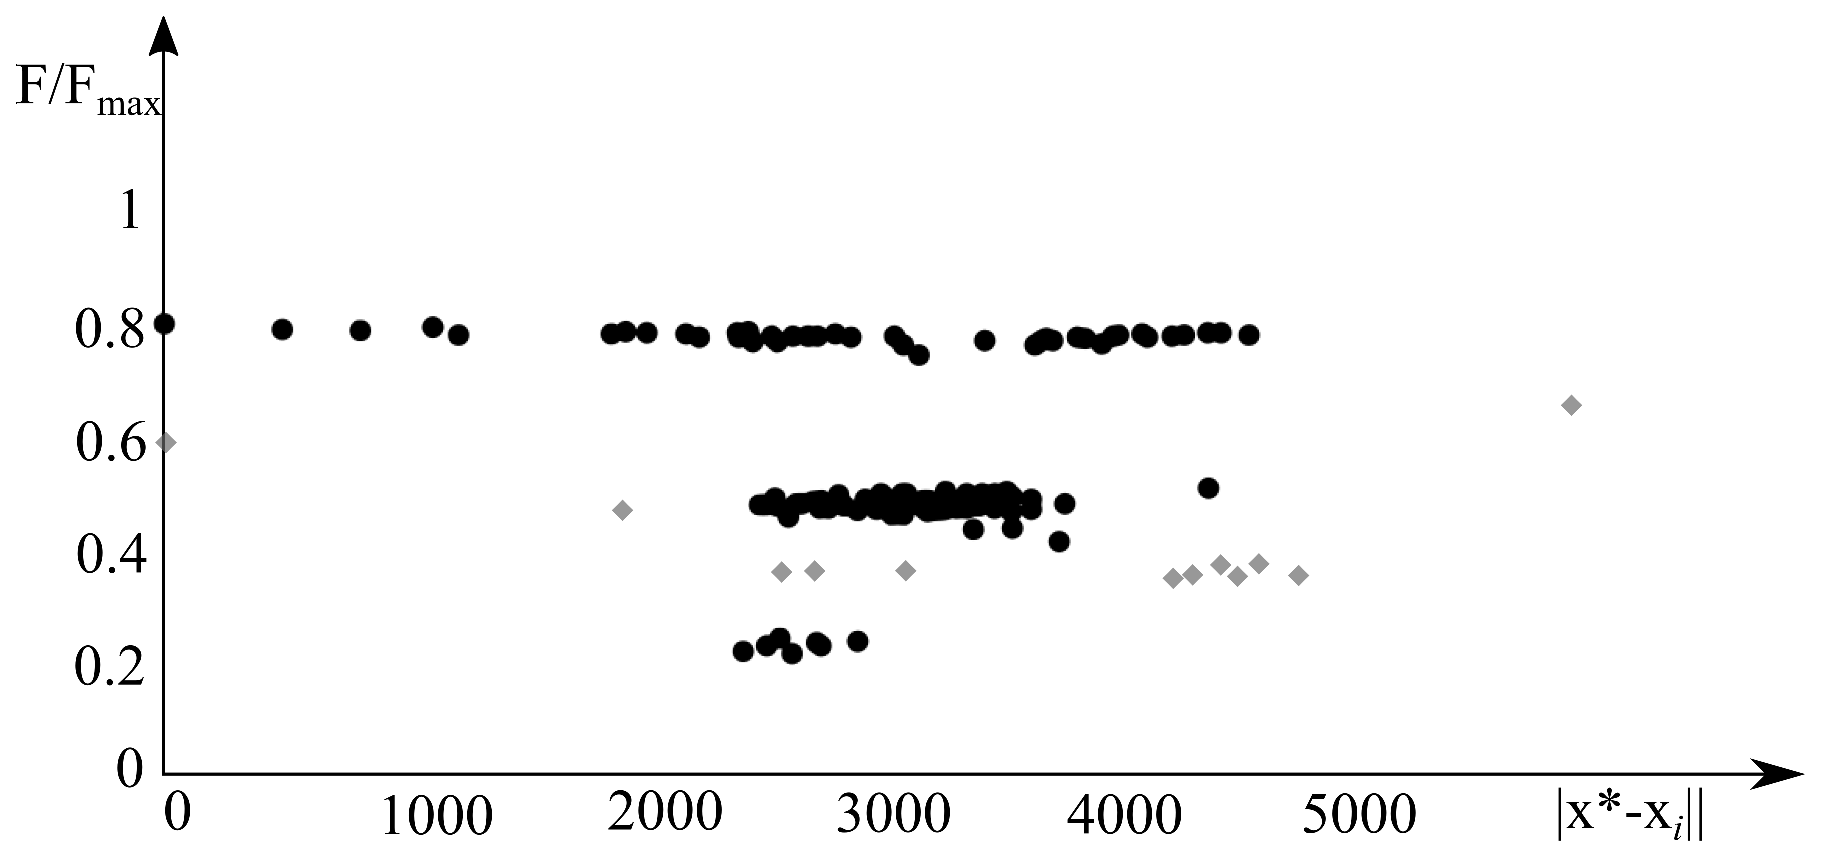
\includegraphics[width=0.9\linewidth]{fit_dist_2x2.eps}  \\ б) }
    \end{minipage}
    \vspace{0.7em}
    \caption{Структура множества найденных решений для задач ШВИ, ШВД, СВД~(а) и~СВД'~(б)}
    \label{ris:fit_dist_0}
\end{figure}

Известно \mycite{yurkov:symmetry}{Юрков~А.С.,~2020}, что любой элемент группы непрерывных симметрий задачи~(\ref{eq:task3_0}) может быть описан в виде~(\ref{eq:sunexp_0}).
\begin{equation}
\label{eq:sunexp_0}
Q=e^{\sum\limits_n a_n G_n} \, .
\end{equation}
где $a_n$ -- вещественные числа, $G_n$ -- генераторы в теоретико-групповом смысле. В качестве генераторов $G_n$ можно выбрать косо-симметричные матрицы, которые содержат над главной диагональю один единичный элемент, симметричный ему противоположный элемент и остальные нули.
Введем матрицу: $ {\textbf{H}}_{\Sigma} = \sum_{i} \textbf{H}_i,$ которая может быть представлена в виде конгруэнтного преобразования диагональной матрицы $D$:
$${\textbf{H}}_{\Sigma} = S^TDS,$$
при некоторой матрице $S$.
Нахождение непрерывных групп симметрий сводится к решению задачи~(\ref{eq:commutat2_0}).

\begin{equation}
\label{eq:commutat2_0}
\left\{
\begin{array}{l}
\displaystyle
\tilde{\textbf{H}}_i \left(\sum\limits_na_nG_n\right) =
\left(\sum\limits_na_nG_n\right)\tilde{\textbf{H}}_i \, , \\ \\
\displaystyle
\tilde{\textbf{G}} \left(\sum\limits_na_nG_n\right) = \left(\sum\limits_na_nG_n\right)\tilde{\textbf{G}} \, .
\end{array}
\right.
\end{equation}

\begin{equation}
\tilde{\textbf{G}}=\left(S^{-1}\right)^T \textbf{A} S^{-1} \, , \qquad
\tilde{\textbf{B}_i}=\left(S^{-1}\right)^T \textbf{B}_i S^{-1} \, , \ i=1,\dots,M.
\end{equation}

Вычислительный эксперимент по поиску группы непрерывных симметрий состоит из следующих этапов:
\begin{enumerate}
  \item Предварительная обработка. Возможная неточность данных нивелируется усреднением симметричных компонент матриц (матрицы $\textbf{G}$ и $\textbf{H}$ должны быть симметричны).
  \item %Normalization of matrices $B_i$.
  Преобразование $ {\textbf{H}}_{\Sigma} = \sum_{i} \textbf{H}_i$ к канонической форме используя метод Лагранжа для вычисления матриц~$S$ и $S^{-1} $.
  \item Применение метода Гаусса к системе линейных уравнений~(\ref{eq:commutat2}) для вычисления генераторов~$\hat{G}_n$.
\end{enumerate}

%\subsection{Optimization of the Excitation of Antenna Arrays}

Описанная процедура нахождения непрерывных групп симметрий применяется к примерам, описанным в главе 1. Для всех рассмотренных задач было выявлено только наличие фазовой симметрии.

{\textbf{Четвертая глава}} посвящена исследованию возможности оптимизации возбуждения ФАР в различных условиях.

На практике использование высокосимметричных ФАР вызывает особый интерес, так как позволяет выполнить расчеты для одного направления и затем легко адаптировать их для других симметричных направлений. Другой особенностью, влияющей на результаты моделирования является наличие потерь в земле \mycite{yurkov:groundloss}{Юрков~А.С.,~2014}. Чтобы ослабить этот эффект, антенные системы с противовесами подняты над землей на 2 м.

В данной главе мы изучаем, как изменяется общий коэффициент усиления кольцевой ФАР с ростом радиочастоты и плотности системы противовесов. Общий коэффициент усиления является суммой частичных коэффициентов усиления в  двух ортогональных поляризациях. Плотность системы противовесов определяется числом продольных и поперечных проводов, относящихся к одному и тому же излучателю. Частота изменяется от 5 до 30 МГц. Вычисления производились на решетках ШВИ, состоящих из 8 излучателей. Для расчета матрицы сопротивлений и матрицы излучений использовался пакет моделирования антенных систем NEC2.

Для проведения вычислительного эксперимента использовался решатель BARON в пакете GAMS. Результаты оптимизации направленности решетки сравниваются с коэффициентом усиления одиночного излучателя, установленного в центре такой же системы противовесов. Плотность системы противовесов обозначается в формате $long:trans$, где $long$ -- число продольных проводов, относящихся к одному излучателю, а $trans$ -- поперечных. Высота каждого ШВИ -- 15м. В качестве направления оптимизации выбирается $70^{\circ}$ полярного угла и $45^{\circ}$ азимутального угла в сферических координатах.

На рис.~\ref{ris:paa_gains_0} показано, как изменяется коэффициент усиления с ростом радиочастоты. Мы можем наблюдать, что при значениях частоты 5 и 30 МГц решетка оптимизируется малоэффективно. Также можно увидеть, что, в основном, увеличение плотности системы противовесов приводит к росту коэффициента усиления.

\begin{figure}[!h]
\center{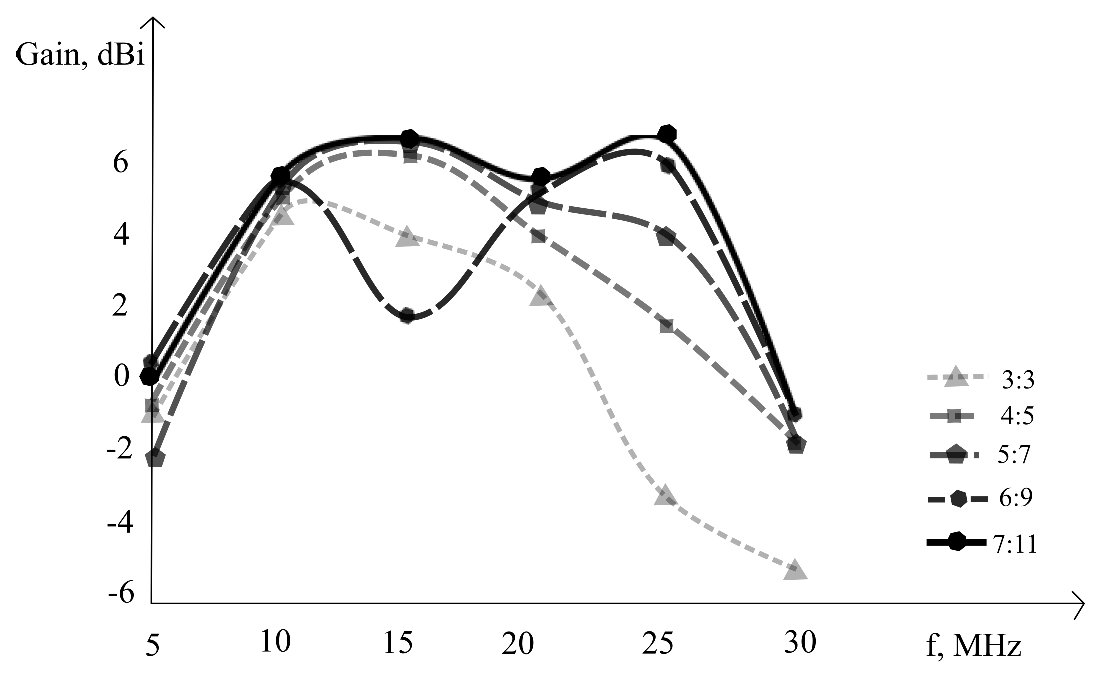
\includegraphics[width=0.8\linewidth]{ring_f__paa_gains.eps}}
\caption{Зависимость от частоты общего коэффициента усиления ФАР при оптимизации в направлении 70:45}
\label{ris:paa_gains_0}
\end{figure}

На рис.~\ref{ris:all_gains_0} показано, как изменяется соотношение коэффициентов усиления ФАР и одиночного излучателя с ростом частоты. Заметным результатом здесь является то, что на частоте 25МГц усиление ФАР существенно больше усиления одиночного излучателя. Объяснение этого эффекта будет приведено далее при сравнении диаграмм направленности.

\begin{figure}[!h]
\center{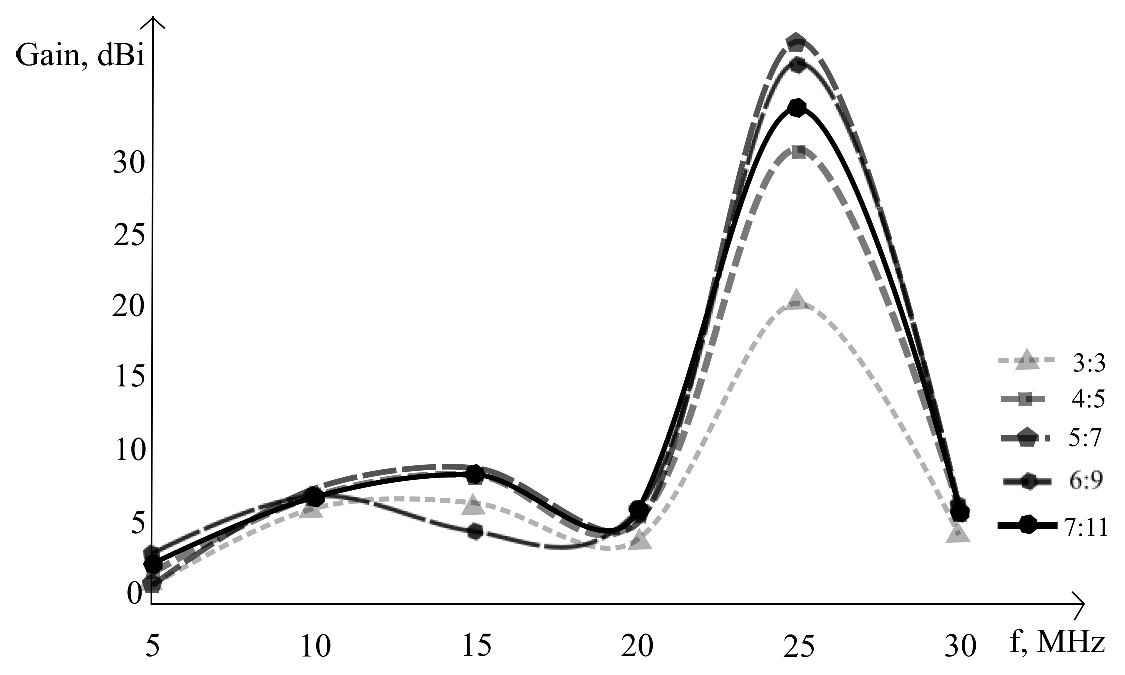
\includegraphics[width=0.8\linewidth]{ring_f_gains.eps}}
\caption{Сравнение коэффициентов усиления ФАР и одиночного излучателя}
\label{ris:all_gains_0}
\end{figure}

На частоте 25МГц (см~Рис.~\ref{ris:f25mhs_0}), где усиление ФАР существенно больше усиления одиночного излучателя. Одиночный излучатель довольно мало излучает в направлении оптимизации, тогда как ФАР имеет максимум излучения в этом направлении. Было предположено, что такой эффект был получен вследствие учета взаимного влияния. Согласно~(\ref{eq:A_0}), если пренебречь взаимным влиянием излучателей, плотность мощности $F$ будет максимальна, когда поля будут синфазны. Для проверки гипотезы о необходимости учета взаимного влияния произведено сравнение диаграмм направленности решеток разных конфигураций после математической оптимизации их направленности в заданном направлении согласно модели~(\ref{eq:task3_0}) с соответствующими диаграммами одиночного излучателя и со случаем фазирования решетки без учета взаимного влияния (далее – простое фазирование).

\begin{figure}[!h]
\begin{minipage}[h]{0.49\linewidth}
\center{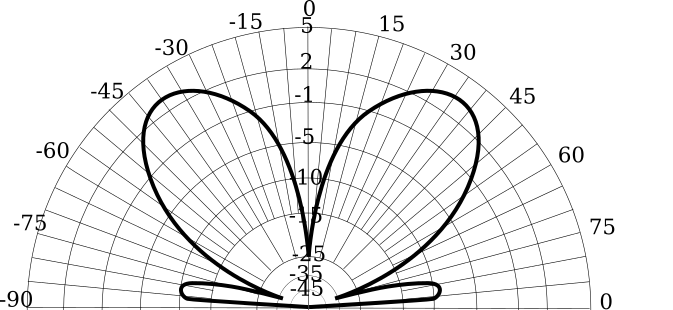
\includegraphics[width=1\linewidth]{r8_1_25_5x7.png} \\ а)}
\end{minipage}
\hfill
\begin{minipage}[h]{0.49\linewidth}
\center{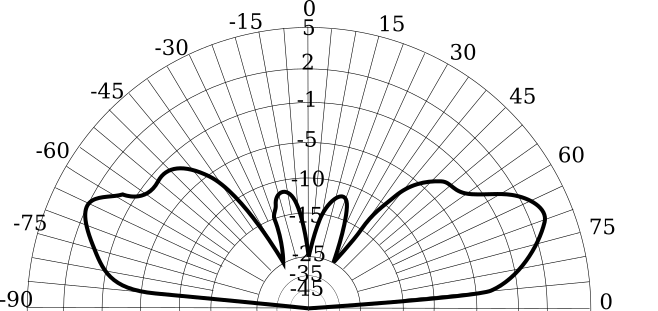
\includegraphics[width=1\linewidth]{r8_25_5x7.png} \\ б)}
\end{minipage}
\caption{Вертикальный план диаграммы направленности одиночного излучателя (а) и ФАР 5:7 (б) при 25МГц}
\label{ris:f25mhs_0}
\end{figure}

Направление оптимизации по умолчанию было установлено на $70^{\circ}$ полярного угла и $45^{\circ}$ азимутального угла в сферических координатах. Для некоторых экспериментов было проведено дополнительное исследование при $85^{\circ}$ полярного угла.


Для ШВД производилось исследование диаграмм направленности при варьировании расстояния центров излучателей до центра решетки от~5 до 50~м. В большинстве случаев, использование решения задачи математического программирования не давало существенного преимущества перед простым фазированием. Тем не менее, при расстоянии между центром излучателя и центром решетки равным 20~м. это различие составило около 4~дБ~(см.~Рис.~\ref{pic:r_bvd_result_0}).

\begin{figure}
\begin{minipage}[h]{0.49\linewidth}
\center{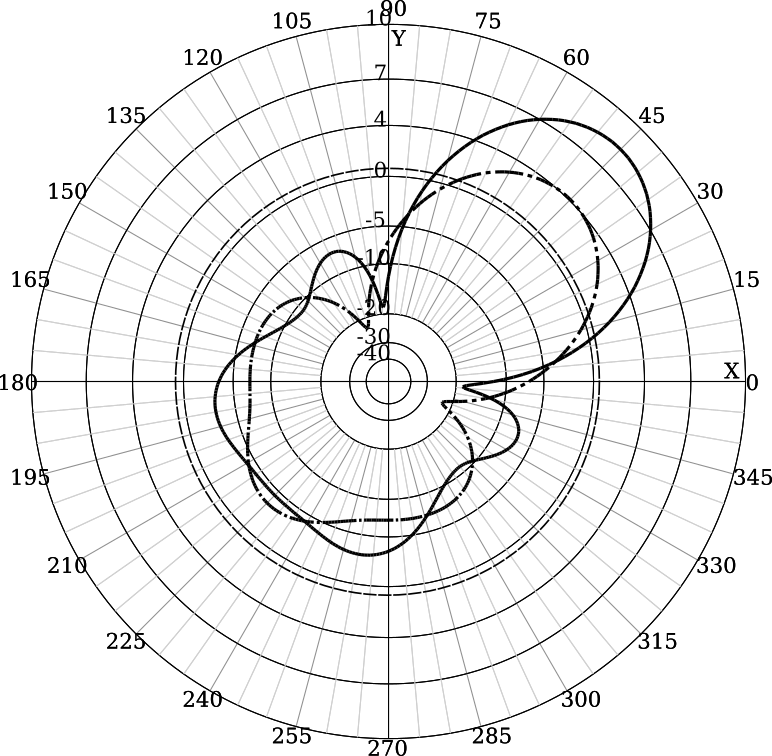
\includegraphics[width=1\linewidth]{r_bvd_20_results_h.png} \\ а)}
\end{minipage}
\hfill
\begin{minipage}[h]{0.49\linewidth}
\center{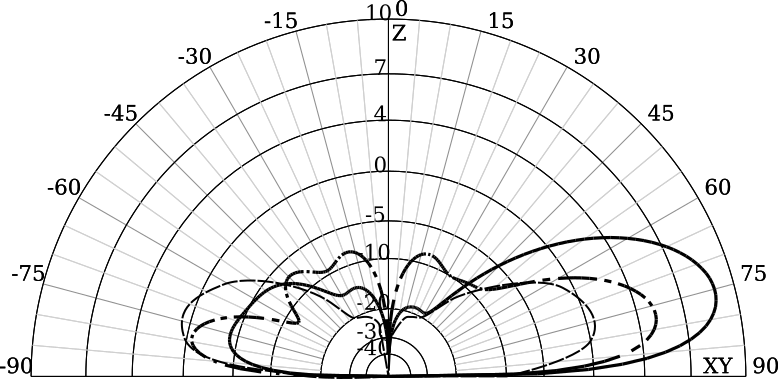
\includegraphics[width=1\linewidth]{r_bvd_20_results_v.png} \\ б)}
\end{minipage}
\caption{Горизонтальный (а) и вертикальный (б) план диаграммы направленности ШВД при расстоянии от центра излучателя до центра решетки 20 м. Пунктирной линией обозначено усиление одиночного излучателя, штрихпунктирной – простое фазирование, сплошной – решение задачи мат. программирования.}
\label{pic:r_bvd_result_0}
\end{figure}

Аналогичные результаты были получены и для решеток~СВД. При оптимизации в направлении полярного угла равном $70^{\circ}$ при варьировании расстояния от центра излучателя до центра решетки от~35 до 37~м. различие между коэффициентом усиления решения задачи математического программирования и усилением простого фазирования также достигало 4~дБ.  При оптимизации в направлении полярного угла равном $85^{\circ}$ при варьировании расстояния от центра излучателя до центра решетки от 25 до 29~м. эта разница достигала 5~дБ.

\FloatBarrier
\pdfbookmark{Заключение}{conclusion}                                  % Закладка pdf
В {\textbf{заключении}} приведены основные результаты работы\ifdisser{, которые заключаются в следующем:
%% Согласно ГОСТ Р 7.0.11-2011:
%% 5.3.3 В заключении диссертации излагают итоги выполненного исследования, рекомендации, перспективы дальнейшей разработки темы.
%% 9.2.3 В заключении автореферата диссертации излагают итоги данного исследования, рекомендации и перспективы дальнейшей разработки темы.
\begin{enumerate}
  \item В текущей работе была рассмотрена постановка задачи оптимизации направленности излучения антенной системы, представленной в виде регулярной решетки излучателей. Для данной задачи была разработана модель квадратичного программирования в вещественных числах. Произведено сравнение результатов разработанных алгоритмов в вычислительном эксперименте.
  \item Проведены вычислительные эксперименты, выявляющие наличие непрерывных групп симметрий допустимых решений. Для всех рассмотренных задач выявлено наличие только фазовой симметрии.
  \item В рамках данного исследования было выявлено наличие ситуаций, в которых коэффициент усиления, соответствующий решению задачи математического программирования, имеет существенное преимущество перед коэффициентом усиления простого фазирования. Выявлено, что, при оптимизации направленности ФАР КВ диапазона целесообразны расчеты с учетом взаимного влияния излучателей.
  \item Для генерации тестовых примеров, автоматизации вычислительных экспериментов и визуализации их результатов были разработаны интерпретатор <<Expi>> и его графическая оболочка <<ExpiIDE>>.
\end{enumerate}

}{.
    \section*{Основные результаты}
    %% Согласно ГОСТ Р 7.0.11-2011:
%% 5.3.3 В заключении диссертации излагают итоги выполненного исследования, рекомендации, перспективы дальнейшей разработки темы.
%% 9.2.3 В заключении автореферата диссертации излагают итоги данного исследования, рекомендации и перспективы дальнейшей разработки темы.
\begin{enumerate}
  \item В текущей работе была рассмотрена постановка задачи оптимизации направленности излучения антенной системы, представленной в виде регулярной решетки излучателей. Для данной задачи была разработана модель квадратичного программирования в вещественных числах. Произведено сравнение результатов разработанных алгоритмов в вычислительном эксперименте.
  \item Проведены вычислительные эксперименты, выявляющие наличие непрерывных групп симметрий допустимых решений. Для всех рассмотренных задач выявлено наличие только фазовой симметрии.
  \item В рамках данного исследования было выявлено наличие ситуаций, в которых коэффициент усиления, соответствующий решению задачи математического программирования, имеет существенное преимущество перед коэффициентом усиления простого фазирования. Выявлено, что, при оптимизации направленности ФАР КВ диапазона целесообразны расчеты с учетом взаимного влияния излучателей.
  \item Для генерации тестовых примеров, автоматизации вычислительных экспериментов и визуализации их результатов были разработаны интерпретатор <<Expi>> и его графическая оболочка <<ExpiIDE>>.
\end{enumerate}

}

%Для проведения вычислительных экспериментов был разработан интерпретатор <<Expi>> и его графическая оболочка <<ExpiIDE>>.

%Формат языка <<Expi>> позволяет в декларативной форме объявлять правила построения моделей и задавать параметры запуска экспериментов.
%В языке <<Expi>> предоставлены возможности моделировать конфигурации проводников в зависимости от динамических параметров, объединять их в группы и применять к ним геометрические преобразования. Также имеется возможность экспорта определенных конфигураций в формат NEC. Отдельно следует отметить возможность языка выполнять серии вычислительных экспериментов. В <<Expi>> уже встроен интерфейс для работы с пакетом GAMS, а также имеется возможность интеграции любого пользовательского пакета.

%Графическая оболочка <<ExpiIDE>> представляет собой файловый инспектор с возможностью редактировать и запускать файлы экспериментов exp, просматривать и экспортировать диаграммы направленности и геометрию антенных систем.
